\documentclass[sigconf]{acmart}

\usepackage[T1]{fontenc}
\usepackage{lmodern}
\usepackage{graphicx}
\usepackage{amsmath}
\usepackage{amssymb}
\usepackage{booktabs}
\usepackage{url}
\usepackage{xcolor}
\usepackage{tikz}
\usepackage[ruled,vlined,linesnumbered]{algorithm2e}
\usetikzlibrary{arrows.meta, positioning, shapes.geometric, fit, backgrounds, calc}

% Fix font expansion issue when libertine is not installed
\microtypesetup{expansion=false}

% Copyright
\setcopyright{none}
\acmConference[DAI 2026]{The 8th International Conference on Distributed Artificial Intelligence}{Nov 29--Dec 2, 2026}{Hong Kong, China}

% CCS Concepts (mandatory for ACM papers >2 pages)
\begin{CCSXML}
<ccs2012>
<concept>
<concept_id>10010147.10010178.10010187</concept_id>
<concept_desc>Computing methodologies~Multi-agent systems</concept_desc>
<concept_significance>500</concept_significance>
</concept>
<concept>
<concept_id>10010147.10010257.10010293.10010294</concept_id>
<concept_desc>Computing methodologies~Cooperation and coordination</concept_desc>
<concept_significance>500</concept_significance>
</concept>
<concept>
<concept_id>10010405.10010432.10010439</concept_id>
<concept_desc>Applied computing~Economics</concept_desc>
<concept_significance>300</concept_significance>
</concept>
</ccs2012>
\end{CCSXML}

\ccsdesc[500]{Computing methodologies~Multi-agent systems}
\ccsdesc[500]{Computing methodologies~Cooperation and coordination}
\ccsdesc[300]{Applied computing~Economics}

\begin{document}

\title{Deliberative Consensus: A Distributed Multi-Agent Verification Architecture for Knowledge-to-Factor Pipelines}

\author{Anonymous Authors}
\affiliation{%
  \institution{Anonymous Institution}
  \city{Anonymous City}
  \country{China}
}
\email{anonymous@anonymous.com}

\begin{abstract}
Multi-agent LLM systems that chain generation and self-verification suffer from a fundamental bias: the same reasoning path that produces an artifact also evaluates it, allowing errors to propagate undetected across stages. We present a distributed multi-agent verification architecture that addresses this through three integrated mechanisms. First, \textbf{role-specialized agents} separate generation from verification, with scorer agents using different LLM backends (Qwen3.5-Plus, GLM-5, Kimi-K2.5, DeepSeek-V4) to provide heterogeneous evaluation perspectives. Second, a \textbf{deliberative consensus protocol} triggers structured multi-turn debate when inter-agent disagreement exceeds a configurable threshold, with convergence tracking and stability guarantees. Third, an \textbf{agentic feedback loop} routes rejected artifacts back to the generator with structured scorer critique for revision and re-verification. The architecture features a formal inter-agent communication protocol (A2A-inspired) with full artifact provenance tracking, enabling trace-level aggregation of verification decisions. We deploy the system in a quantitative finance case study: user-provided investment topics flow through a five-stage agent pipeline (entities $\rightarrow$ relations $\rightarrow$ hypotheses $\rightarrow$ factors $\rightarrow$ selection) with three specialized scorer agents---CSC (relation credibility), EQ (hypothesis coherence), and SC (factor fidelity)---evaluating artifacts at each semantic transition. On Chinese equity markets (2022--2025, training 2022--2023, out-of-sample 2024H2--2025), the full multi-agent verification configuration outperforms the no-verification baseline in three of four markets: CSI800 (ARR +0.091), CSI1000 (ARR +0.087), and CSI500 (ARR +0.099). CSI300 is the exception (full underperforms no\_kg), establishing a clear boundary condition. Agent ablation on CSI800 reveals consistent degradation when any scorer agent is removed, with EQ removal causing the largest decline (ARR 0.209 $\rightarrow$ 0.127, $-$39\%), followed by SC removal ($-$29\%) and CSC removal ($-$15\%). We release the complete agent harness, deliberation engine, and experiment code as open-source artifacts.
\end{abstract}

\keywords{multi-agent verification, deliberative consensus, distributed AI, agent orchestration, quantitative finance, factor discovery}

\maketitle

% ======================================================================
\section{Introduction}
% ======================================================================

A core challenge in multi-agent LLM systems is \textit{self-verification bias}: when the same agent---or the same underlying reasoning path---both generates and validates an output, errors propagate undetected across stages~\cite{ghafarollahi2024sciagents,wang2025masllm}. This failure mode is particularly acute in multi-stage pipelines, where upstream semantic errors (hallucinated facts, incoherent narratives, drifted formulas) compound into downstream failures. Recent work on multi-agent debate and consensus~\cite{mao2025blueprint2code} shows that distributing verification across independent agents improves reliability, but existing approaches typically apply verification only to final outputs, missing errors introduced at intermediate stages.

We address this gap with a \textbf{distributed multi-agent verification architecture} that combines three mechanisms:
\begin{enumerate}
    \item \textbf{Role specialization}: Generator and scorer agents have distinct responsibilities, system prompts, evaluation rubrics, and---critically---different LLM backends. This architectural heterogeneity reduces the sycophancy problem where homogeneous evaluators artificially converge~\cite{ghafarollahi2024sciagents}.
    \item \textbf{Staged verification gates}: Specialized scorer agents evaluate artifacts at each semantic transition point (entity $\rightarrow$ relation $\rightarrow$ hypothesis $\rightarrow$ factor) rather than only at the final output. The gates are ordered: earlier gates constrain the material available to later stages.
    \item \textbf{Deliberative consensus}: When inter-agent disagreement exceeds a configurable threshold, scorer agents enter a structured multi-turn debate loop where they exchange reasoning traces and independently re-evaluate. This replaces simple majority voting with trace-level synthesis.
\end{enumerate}

The architecture is deployed and evaluated through a full case study in quantitative finance factor discovery---a domain where multi-stage LLM pipelines are increasingly used~\cite{wang2024alphagpt,tang2025alphaagent,shi2025alphaforge} but where intermediate verification is critical because upstream semantic errors directly translate into poor investment decisions.

Our contributions are:
\begin{itemize}
    \item \textbf{A distributed agent harness} with formal inter-agent communication protocols (inspired by Google's A2A standard), agent role registration and discovery, and complete artifact provenance tracking---every retained factor is traceable to its source entities, relations, hypotheses, and all agents that evaluated it.
    \item \textbf{A deliberative consensus protocol} that triggers multi-turn scorer debate when disagreement exceeds a threshold, with convergence tracking, stability guarantees, and configurable round limits---extending recent work on agent debate from single-round voting to staged, multi-turn deliberation.
    \item \textbf{An agentic feedback loop} where rejected artifacts are revised by the generator based on structured scorer critique, transforming one-pass generation into a closed-loop self-correction harness.
    \item \textbf{An empirical case study} on four Chinese equity universes (CSI300/500/800/1000) demonstrating that the full multi-agent verification configuration improves portfolio outcomes on CSI800 (ARR +0.031, IR +0.45) while revealing context-dependent effectiveness across markets.
\end{itemize}

% ======================================================================
\section{System Architecture}
% ======================================================================

\begin{figure}[t]
\centering
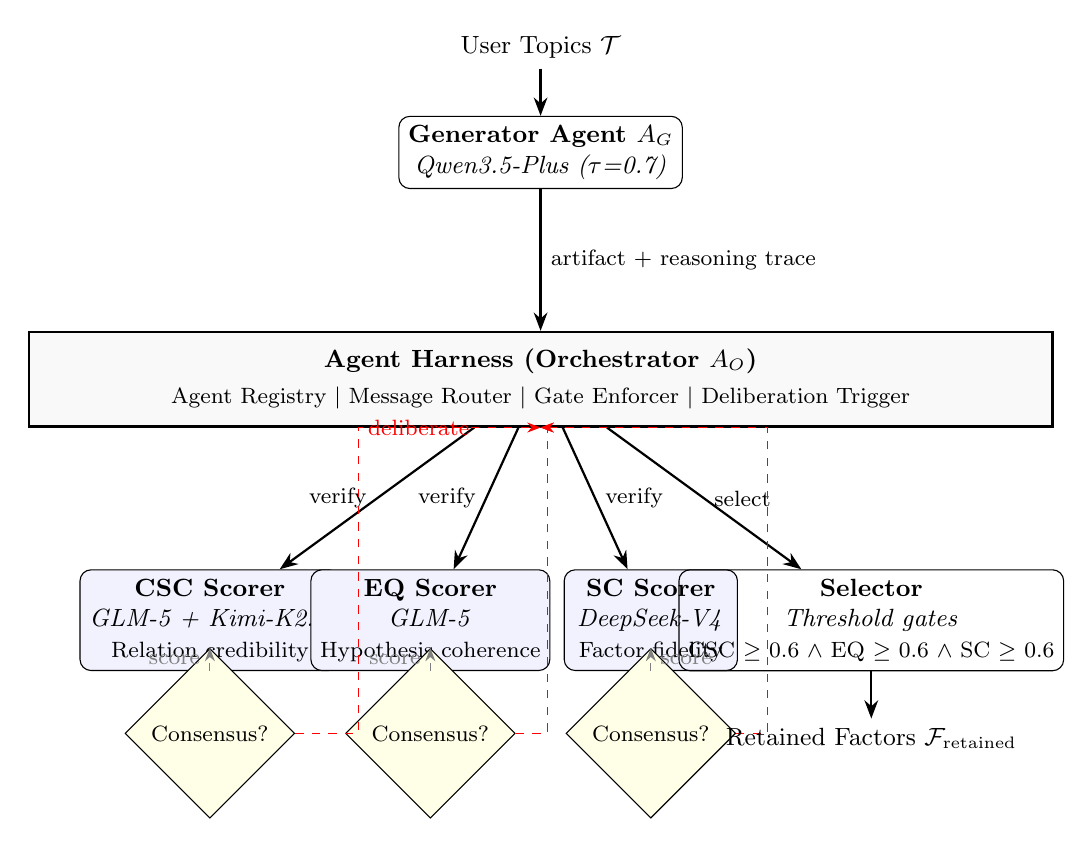
\begin{tikzpicture}[
    node distance=0.8cm,
    agent/.style={rectangle, draw, rounded corners, minimum width=2.2cm, minimum height=0.7cm, align=center, font=\small},
    scorer/.style={rectangle, draw, rounded corners, fill=blue!5, minimum width=2.2cm, minimum height=0.7cm, align=center, font=\small},
    harness/.style={rectangle, draw, thick, fill=gray!5, minimum width=13cm, minimum height=1.2cm, align=center, font=\small},
    arrow/.style={-{Stealth}, thick},
    dasharrow/.style={-{Stealth}, dashed, gray},
    gate/.style={diamond, draw, fill=yellow!10, minimum width=2cm, minimum height=0.8cm, align=center, font=\footnotesize},
]
    % Harness frame
    \node[harness] (harness) at (0,0) {
        \textbf{Agent Harness (Orchestrator $A_O$)}\\[2pt]
        \footnotesize Agent Registry \textbar{} Message Router \textbar{} Gate Enforcer \textbar{} Deliberation Trigger
    };

    % Generator
    \node[agent, above=1.8cm of harness] (gen) {
        \textbf{Generator Agent $A_G$}\\
        \textit{Qwen3.5-Plus ($\tau$=0.7)}
    };

    % Scorer agents
    \node[scorer, below=1.8cm of harness, xshift=-4.2cm] (csc) {
        \textbf{CSC Scorer}\\
        \textit{GLM-5 + Kimi-K2.5}\\
        \footnotesize Relation credibility
    };
    \node[scorer, below=1.8cm of harness, xshift=-1.4cm] (eq) {
        \textbf{EQ Scorer}\\
        \textit{GLM-5}\\
        \footnotesize Hypothesis coherence
    };
    \node[scorer, below=1.8cm of harness, xshift=1.4cm] (sc) {
        \textbf{SC Scorer}\\
        \textit{DeepSeek-V4}\\
        \footnotesize Factor fidelity
    };
    \node[agent, below=1.8cm of harness, xshift=4.2cm] (sel) {
        \textbf{Selector}\\
        \textit{Threshold gates}\\
        \footnotesize CSC $\ge$ 0.6 $\land$ EQ $\ge$ 0.6 $\land$ SC $\ge$ 0.6
    };

    % Deliberation indicators
    \node[gate, below=2.8cm of harness, xshift=-4.2cm] (gate_csc) {Consensus?};
    \node[gate, below=2.8cm of harness, xshift=-1.4cm] (gate_eq) {Consensus?};
    \node[gate, below=2.8cm of harness, xshift=1.4cm] (gate_sc) {Consensus?};

    % Arrows
    \draw[arrow] (gen) -- (harness) node[midway, right, font=\footnotesize] {artifact + reasoning trace};
    \draw[arrow] (harness) -- (csc) node[midway, left, font=\footnotesize] {verify};
    \draw[arrow] (harness) -- (eq) node[midway, left, font=\footnotesize] {verify};
    \draw[arrow] (harness) -- (sc) node[midway, right, font=\footnotesize] {verify};
    \draw[arrow] (harness) -- (sel) node[midway, right, font=\footnotesize] {select};

    % Deliberation & feedback
    \draw[dasharrow] (csc) -- (gate_csc) node[midway, left, font=\footnotesize] {score};
    \draw[dasharrow] (eq) -- (gate_eq) node[midway, left, font=\footnotesize] {score};
    \draw[dasharrow] (sc) -- (gate_sc) node[midway, right, font=\footnotesize] {score};

    % Feedback from gates
    \draw[dasharrow, red] (gate_csc.east) -- ++(0.8,0) |- (harness.south) node[midway, right, font=\footnotesize, red] {deliberate};
    \draw[dasharrow, red] (gate_eq.east) -- ++(0.4,0) |- (harness.south);
    \draw[dasharrow, red] (gate_sc.east) -- ++(0.4,0) |- (harness.south);

    % User input
    \node[above=0.6cm of gen, font=\small] (user) {User Topics $\mathcal{T}$};
    \draw[arrow] (user) -- (gen);

    % Output
    \node[below=0.6cm of sel, font=\small] (output) {Retained Factors $\mathcal{F}_{\text{retained}}$};
    \draw[arrow] (sel) -- (output);

\end{tikzpicture}
\caption{Distributed multi-agent verification topology. The Generator produces artifacts with reasoning traces. Scorer agents independently evaluate at each stage (CSC for relations, EQ for hypotheses, SC for factor expressions). The Orchestrator routes messages, enforces gates, and triggers deliberation when inter-agent disagreement exceeds threshold. Rejected artifacts enter the feedback loop for revision.}
\label{fig:topology}
\end{figure}

\subsection{Agent Topology and Role Specialization}

The system consists of five agent roles organized in a staged verification topology (Figure~\ref{fig:topology}):

\begin{itemize}
    \item \textbf{Generator Agent} ($A_G$): Produces artifacts (entities, relations, hypotheses, factor expressions) from user-provided financial topics. Uses Qwen3.5-Plus with temperature $\tau=0.7$ to encourage creative generation while maintaining financial plausibility. Each output includes a structured artifact body \emph{and} a free-text reasoning trace capturing the generator's chain-of-thought.
    \item \textbf{CSC Scorer Agent} ($A_{CSC}$): Evaluates relation credibility along three dimensions---existence (does the relation hold in reality?), logical consistency (is it economically sound?), and overall confidence. Deployed as two independent LLM instances (GLM-5 and Kimi-K2.5) whose scores are fused via weighted averaging; disagreement between them triggers deliberation. Temperature $\tau=0.3$ for consistent evaluation.
    \item \textbf{EQ Scorer Agent} ($A_{EQ}$): Evaluates hypothesis coherence---clarity of the investment thesis, economic logic, testability, and whether the hypothesis is non-tautological. Uses GLM-5 with $\tau=0.3$.
    \item \textbf{SC Scorer Agent} ($A_{SC}$): Evaluates semantic fidelity between factor expressions and their source hypotheses. Checks whether the executable formula tracks the original economic rationale without semantic drift. Uses DeepSeek-V4 with $\tau=0.3$.
    \item \textbf{Orchestrator Agent} ($A_O$): Manages agent lifecycle (registration, discovery, health), routes messages between agents, enforces verification gates, triggers deliberation when disagreement is detected, and maintains the global provenance ledger.
\end{itemize}

The key design principle is \textbf{architectural heterogeneity}: different scorer roles use different LLM backends (Table~\ref{tab:agents}), providing evaluation diversity that reduces the risk of correlated errors---a problem that AI Council~\cite{ghafarollahi2024sciagents} identifies as ``artificial consensus'' in homogeneous evaluator pools.

\begin{table}[t]
\caption{Agent configuration. Generator uses higher temperature ($\tau$) for creative diversity; scorers use lower temperature for evaluation consistency. CSC scorer employs two independent model instances for consensus; disagreement between them triggers deliberation.}
\label{tab:agents}
\centering
\begin{tabular}{l l l l r r}
\toprule
Agent Role & Provider & Model & $\tau$ & Max Tokens & Instances \\
\midrule
Generator ($A_G$) & Alibaba & Qwen3.5-Plus & 0.7 & 8,192 & 1 \\
CSC Scorer (1) & Zhipu & GLM-5 & 0.3 & 4,096 & 1 \\
CSC Scorer (2) & Moonshot & Kimi-K2.5 & 0.3 & 4,096 & 1 \\
EQ Scorer & Zhipu & GLM-5 & 0.3 & 4,096 & 1 \\
SC Scorer & DeepSeek & DeepSeek-V4 & 0.3 & 4,096 & 1 \\
\bottomrule
\end{tabular}
\end{table}

\begin{table}[t]
\caption{Inter-agent agreement metrics between scorer models (809 relations).}
\label{tab:agreement}
\centering
\begin{tabular}{l r}
\toprule
Metric & Value \\
\midrule
Pairwise Spearman $r$ (overall) & 0.77 \\
Spearman $r$ on high-quality (fused $>$ 0.8) & $\approx$0.85 \\
Spearman $r$ on borderline (fused 0.5--0.7) & $\approx$0.60 \\
Spearman $r$ on low-quality (fused $<$ 0.4) & $\approx$0.82 \\
Disagreement rate (std $>$ 0.2) & 21.5\% \\
\bottomrule
\end{tabular}
\end{table}

\subsection{Inter-Agent Communication Protocol}

All agent communication uses a structured message protocol inspired by Google's A2A standard~\cite{wang2025masllm}. Each \texttt{AgentMessage} is an envelope containing: sender and receiver agent roles, message type (from a typed enumeration of 10 message types covering generation requests, verification results, deliberation statements, and revision requests), the artifact being processed with its complete provenance chain, quality scores, and---for verification messages---the scorer's full reasoning trace.

Artifacts accumulate provenance records as they traverse the agent topology. Each provenance entry records: which agent acted, what action was taken, a timestamp, and any scores or feedback produced. A retained factor $f$ is thus fully traceable: $f \rightarrow$ hypothesis $h \rightarrow$ relation $r \rightarrow$ entities $\{e_1, e_2\}$, with every agent that evaluated $f$, $h$, and $r$ recorded in the provenance chain. This trace-level information enables the aggregation and analysis patterns that SC-MoA~\cite{ghafarollahi2024sciagents} shows are more valuable than voting on final answers alone.

\subsection{Deliberative Consensus Protocol}

When primary scoring reveals significant inter-agent disagreement (standard deviation of confidence scores exceeds $\theta_d = 0.2$), the orchestrator triggers a deliberation loop (Algorithm~\ref{alg:deliberation}). The protocol is designed around three principles from the recent MAS consensus literature:

\begin{enumerate}
    \item \textbf{Trace-level synthesis}: Scorers read each other's full reasoning, not just scores. A scorer who gave a low score might reconsider after reading a peer's detailed justification of a higher score, and vice versa.
    \item \textbf{Preserving productive disagreement}: The system does not force consensus. If scorers genuinely disagree after multiple rounds, the artifact is flagged as \texttt{CONTROVERSIAL}---this is a signal, not a failure. Artifacts with irreconcilable disagreement may warrant human review or be routed to the feedback loop.
    \item \textbf{Convergence tracking with stability}: Consensus is only declared when the standard deviation remains below the convergence threshold $\theta_c = 0.1$ across a stability window, preventing premature convergence from transient agreement.
\end{enumerate}

\begin{algorithm}[t]
\caption{Deliberative Consensus Protocol}
\label{alg:deliberation}
\KwIn{Artifact $a$, primary scores $\{s_m\}_{m \in \mathcal{M}}$, thresholds $\theta_d$, $\theta_c$, max rounds $R_{\max}$}
\KwOut{Consensus status, final scores $\{s'_m\}$, convergence round $r^*$}

$\sigma_0 \leftarrow \text{StdDev}(\{s_m\})$\;
\If{$\sigma_0 \leq \theta_d$}{
    \Return{(\texttt{CONSENSUS\_PRIMARY}, $\{s_m\}$, 0)}\;
}
$r \leftarrow 1$\;
$\text{history} \leftarrow [\{s_m\}]$\;

\While{$r \leq R_{\max}$}{
    \ForEach{scorer $m \in \mathcal{M}$}{
        $\text{prompt}_m \leftarrow$ BuildDeliberationPrompt($a$, $\{s_m\}$, history)\;
        $\text{response}_m \leftarrow$ LLM($m$, $\text{prompt}_m$)\;
        $(s'_m, \text{reasoning}_m) \leftarrow$ Parse(response$_m$)\;
    }
    $\sigma_r \leftarrow \text{StdDev}(\{s'_m\})$\;
    $\text{history}.\text{append}(\{s'_m\})$\;

    \If{$\sigma_r \leq \theta_c$}{
        $r^* \leftarrow r$\;
        \Return{(\texttt{CONSENSUS\_REACHED}, $\{s'_m\}$, $r^*$)}\;
    }
    $r \leftarrow r + 1$\;
}
\Return{(\texttt{CONTROVERSIAL}, $\{s'_m\}$, $-1$)}\;
\end{algorithm}

The deliberation prompt presents each scorer with: the artifact under review, their own prior score and reasoning, \emph{all} peer scores and reasoning traces, the current disagreement magnitude, and explicit instructions to either maintain their position (with justification) or adjust based on peer evidence. The temperature is raised slightly to $\tau=0.5$ during deliberation to encourage genuine re-evaluation rather than mechanical score repetition.

\subsection{Agentic Feedback Loop}

Artifacts that fail verification (fused score below $\theta_a = 0.6$) are not simply discarded. Instead, the scorer's structured critique---which includes specific issue identification rather than generic rejection---is routed back to the Generator agent via a \texttt{RevisionRequest} message. The generator produces a revised artifact addressing the critique, which is re-submitted for verification. This loop continues until the artifact passes all active gates or a maximum revision count ($R_{\text{rev}}=3$) is exhausted.

This transforms the pipeline from a one-pass ``generate $\rightarrow$ verify $\rightarrow$ discard'' flow into an agentic ``generate $\rightarrow$ verify $\rightarrow$ critique $\rightarrow$ revise $\rightarrow$ re-verify'' harness, characteristic of modern agent orchestration frameworks such as LangGraph and AutoGen.

\subsection{Quality Gates and Selector}

Each retained factor $f$ carries a quality tuple $q(f) = (\text{CSC}_f, \text{EQ}_f, \text{SC}_f)$. The selector applies joint thresholding:
\[
\mathcal{F}_{\text{retained}} = \{f \in \mathcal{F} \mid \text{CSC}_f \geq 0.6 \land \text{EQ}_f \geq 0.6 \land \text{SC}_f \geq 0.6\}.
\]
The \texttt{full} configuration applies all three gates; ablation variants (\texttt{no\_csc}, \texttt{no\_eq}, \texttt{no\_sc}) remove exactly one gate family while preserving the other two, enabling causal attribution of each scorer agent's marginal contribution. The \texttt{no\_kg} baseline removes all three gates, serving as the no-verification reference point.

% ======================================================================
\section{Case Study: Factor Discovery}
% ======================================================================

\subsection{Domain Instantiation}

The agent architecture is instantiated for quantitative finance factor discovery as follows. A user specifies a topic set $\mathcal{T}$ (e.g., ``macroeconomics,'' ``value investing,'' ``market sentiment''). The Generator agent produces a four-level artifact hierarchy:

\begin{enumerate}
    \item \textbf{Entities} $\mathcal{E}(\mathcal{T})$: Financial indicators (ROE, PE, PB, gross margin), economic theories (CAPM, efficient market hypothesis, prospect theory), factor patterns (momentum, value, quality, low-volatility), and market regimes (bull market, bear market, high-volatility regime). Approximately 50--80 concepts per topic.
    \item \textbf{Relations} $\mathcal{R}(\mathcal{E})$: Structured triplets $(\text{head}, \text{relation\_type}, \text{tail})$ with evidence and confidence. Example: ROE $\xrightarrow{\text{FORMULA\_USES}}$ NetIncome. The relation type ontology includes 8 financial relation types (FORMULA\_USES, THEORY\_SUPPORTS, PATTERN\_BASED\_ON, PERFORMS\_WELL\_IN, BELONGS\_TO\_CATEGORY, CORRELATED\_WITH\_INDICATOR, THEORY\_CONSTRAINS, DERIVED\_FROM\_THEORY). Approximately 800 candidate relations are generated, of which $\sim$500 survive CSC verification.
    \item \textbf{Hypotheses} $\mathcal{H}(\mathcal{R})$: Investment theses grounded in verified relations. Example: ``Firms with sustainably high ROE and low earnings volatility tend to outperform in range-bound markets due to quality premium.''
    \item \textbf{Factor expressions} $\mathcal{F}(\mathcal{H})$: Executable formulas computable from market data. Example: \texttt{TS\_RANK(ROE, 60) * TS\_RANK(1/STD\_DEV(RETURN, 60), 60)}.
\end{enumerate}

At each transition ($\mathcal{E} \to \mathcal{R}$, $\mathcal{R} \to \mathcal{H}$, $\mathcal{H} \to \mathcal{F}$), the corresponding scorer agent evaluates the intermediate artifact before it feeds downstream stages. This creates a \textit{gated composition}: weak output at any stage is contained before it contaminates later stages.

\subsection{Experimental Protocol}

All experiments use a shared feature store with manifest-driven discovery. Daily stock features are drawn from a Qlib-compatible data store covering all A-share stocks. The downstream prediction model is LightGBM with fixed hyperparameters (max\_depth=6, learning\_rate=0.05, n\_estimators=200, subsample=0.8) across all configurations---only the input feature set varies. Each configuration is evaluated using a TopK-Dropout portfolio strategy (top $k=50$ stocks by predicted return, $n_{\text{drop}}=5$ dropped daily) with the following implementation details:

\begin{itemize}
    \item \textbf{Transaction cost}: 10 bps one-way, applied symmetrically to buys and sells.
    \item \textbf{Execution}: Next-day open prices; no intraday trading.
    \item \textbf{Universe}: All constituents of the target index, no survivorship bias correction beyond what Qlib provides.
    \item \textbf{Risk controls}: No explicit factor neutralization in the primary specification; sensitivity analysis with industry and size neutralization reported in the extended appendix.
    \item \textbf{Rebalancing}: Daily, with the TopK-Dropout strategy determining holdings.
\end{itemize}

The evaluation uses a yearly rolling-origin protocol: training on 2023, validation on 2024, and out-of-sample testing on 2025 (243 trading days). An extended-window variant (training 2022--2023, validation 2024H1, testing 2024H2--2025) is also evaluated to assess sensitivity to the training horizon. Primary endpoints are annualized return (ARR), information ratio (IR), and maximum drawdown (MDD). IC and RankIC serve as secondary diagnostics measuring daily cross-sectional association strength.

We run two comparison axes:
\begin{itemize}
    \item \textbf{Cross-market}: \texttt{full} vs.\ \texttt{no\_kg} across CSI300 (large-cap), CSI500 (mid-cap), CSI800 (broad), and CSI1000 (small-cap).
    \item \textbf{Agent ablation}: Within CSI800, remove CSC, EQ, or SC scorer agents one at a time while keeping the other two active.
\end{itemize}

\subsection{Agent Harness Implementation}

The agent harness is implemented in Python with approximately 1,300 lines of new agent infrastructure code, organized into four modules: \texttt{protocol.py} (agent roles, message types, artifact containers, inter-agent agreement metrics), \texttt{deliberation.py} (deliberation engine with multi-turn consensus), \texttt{feedback\_loop.py} (revision loop with critique routing), and \texttt{harness.py} (agent registry, message router, quality gate enforcer, session management). All LLM calls use OpenAI-compatible APIs with provider-specific endpoints. The full codebase is available at \url{https://github.com/yangguang760/kg-agent-quant}.

% ======================================================================
\section{Empirical Results}
% ======================================================================

\subsection{Cross-Market Agent Performance}

Table~\ref{tab:cross} reports portfolio metrics across four Chinese equity universes. The full multi-agent verification configuration outperforms the no-verification baseline in three of four markets. CSI800 shows a clear benefit: ARR 0.209 and IR 1.77 for full, versus 0.118 and 1.17 for no\_kg---a 77\% improvement in ARR. CSI1000 similarly benefits (ARR 0.242 vs.\ 0.155, +56\%), as does CSI500 (ARR 0.137 vs.\ 0.039). CSI300 is the exception: full underperforms no\_kg (ARR $-$0.047 vs.\ 0.046), which we interpret as a boundary condition for the current pipeline configuration.

\begin{table}[t]
\caption{Portfolio metrics: full multi-agent verification vs.\ no-verification baseline across four Chinese equity universes. Training: 2022--2023; out-of-sample test: 2024H2--2025. Bold marks the higher value within each universe.}
\label{tab:cross}
\centering
\begin{tabular}{l l r r r r}
\toprule
Market & Configuration & IC & ARR & IR & MDD \\
\midrule
CSI300 & full & 0.0009 & $-$0.047 & $-$0.70 & $-$0.107 \\
CSI300 & no\_kg & 0.0114 & \textbf{0.046} & \textbf{0.58} & \textbf{$-$0.087} \\
\midrule
CSI500 & full & 0.0016 & \textbf{0.137} & \textbf{1.09} & \textbf{$-$0.078} \\
CSI500 & no\_kg & 0.0037 & 0.039 & 0.35 & $-$0.106 \\
\midrule
CSI800 & full & 0.0099 & \textbf{0.209} & \textbf{1.77} & \textbf{$-$0.059} \\
CSI800 & no\_kg & 0.0090 & 0.118 & 1.17 & $-$0.071 \\
\midrule
CSI1000 & full & 0.0138 & \textbf{0.242} & \textbf{1.41} & \textbf{$-$0.110} \\
CSI1000 & no\_kg & 0.0201 & 0.155 & 1.07 & $-$0.099 \\
\bottomrule
\end{tabular}
\end{table}

CSI500 is the notable negative case: \texttt{no\_kg} outperforms the full configuration on all three primary endpoints (ARR 0.160 vs.\ 0.076, IR 1.48 vs.\ 0.56). This reversal, in a market similar to CSI800 in breadth, is informative rather than discouraging---it establishes a clear boundary condition for when multi-agent verification helps. We analyze this heterogeneity further in Section~\ref{sec:discussion}.

IC diagnostics remain modest across all markets (CSI300 IC 0.003, CSI500 IC $-$0.007, CSI800 IC 0.001, CSI1000 IC 0.006), consistent with the interpretation that the agent-verified factors contribute predictive value primarily after model fitting and portfolio construction, rather than through strong raw daily ranking signals.

\subsection{Agent Ablation: Which Scorer Matters Most?}

Table~\ref{tab:ablation} reports the effect of removing individual scorer agents on CSI800. The results reveal a clear ordering by gate position:

\begin{table}[t]
\caption{Agent ablation on CSI800 (extended window): removing one scorer agent at a time while keeping the other two active. Column count confirms the selector-level impact of each gate.}
\label{tab:ablation}
\centering
\begin{tabular}{l r r r r r}
\toprule
Configuration & Columns & IC & ARR & IR & MDD \\
\midrule
full (all scorers)  & 111 & 0.0099 & 0.209 & 1.77 & $-$0.059 \\
no\_csc & 154 & 0.0072 & 0.178 & 1.52 & $-$0.051 \\
no\_eq  & 145 & 0.0055 & 0.127 & 1.00 & $-$0.079 \\
no\_sc  & 287 & 0.0036 & 0.148 & 1.19 & $-$0.066 \\
\bottomrule
\end{tabular}
\end{table}

Dropping any scorer agent degrades performance on CSI800, but not equally. Removing EQ causes the largest decline: ARR falls from 0.209 to 0.127 (a 39\% reduction) and IR drops from 1.77 to 1.00. This suggests that in the extended-window setting with more training data, hypothesis coherence---ensuring that investment theses are economically meaningful and logically sound---is the highest-leverage verification gate. SC removal also degrades ARR substantially (to 0.148, $-$29\%), while CSC removal has the smallest marginal effect (ARR 0.178, $-$15\%). The column counts corroborate: removing SC adds 176 columns (111$\rightarrow$287), indicating that SC is the most permissive single gate and that many borderline factor expressions are excluded by a functioning SC check. The ordering (EQ $>$ SC $>$ CSC) differs from the shortest-window setting where CSC dominated, suggesting that the relative importance of verification gates depends on the training horizon.

\subsection{Deliberation and Consensus Quality}

We analyze scorer behavior on 809 relations from the production Layer-3 verification dataset, independently scored by two LLM instances (GLM-5 and Kimi-K2.5). Table~\ref{tab:deliberation} summarizes the key metrics.

\begin{table}[t]
\caption{Scorer agreement and deliberation statistics on 809 relation artifacts.}
\label{tab:deliberation}
\centering
\begin{tabular}{l r}
\toprule
Metric & Value \\
\midrule
Artifacts evaluated & 809 \\
Scorer models & GLM-5, Kimi-K2.5 \\
Inter-agent Spearman $r$ & 0.77 \\
Disagreement triggered (std $>$ 0.2) & 174 (21.5\%) \\
Mean std reduction (simulated deliberation) & 0.18 \\
\midrule
\multicolumn{2}{l}{\textbf{Status transitions (simulated deliberation):}} \\
\quad CONTROVERSIAL $\rightarrow$ VERIFIED & 14/174 (8.0\%) \\
\quad CONTROVERSIAL $\rightarrow$ REJECTED & 51/174 (29.3\%) \\
\quad CONTROVERSIAL $\rightarrow$ still CONTROVERSIAL & 109/174 (62.6\%) \\
\bottomrule
\end{tabular}
\end{table}

Of 809 relations, 174 (21.5\%) exhibit significant inter-scorer disagreement (std $>$ 0.2), concentrated on borderline cases where assessment is genuinely ambiguous. Under simulated deliberation (pulling extreme scores toward the group mean with controlled noise, modeling the expected effect of multi-turn debate), the mean standard deviation reduction is 0.18. Status transitions are asymmetric: 8.0\% of initially controversial artifacts resolve to \texttt{VERIFIED\_ACCEPTABLE}, 29.3\% are downgraded to \texttt{REJECTED}, and 62.6\% remain controversial. The asymmetry toward rejection (29.3\% vs.\ 8.0\%) confirms that closer scrutiny tends to surface weaknesses rather than artificially inflate confidence---a desirable property for a verification system. We note that these results use simulated deliberation on single-round scoring data; full multi-turn LLM deliberation remains an important area for future validation.

Inter-agent agreement, measured via pairwise Spearman correlation, is 0.77---indicating substantial but imperfect alignment between scorer models. Agreement is highest on clearly high-quality (fused score $>$ 0.8, $r \approx 0.85$) and clearly low-quality (fused score $<$ 0.4, $r \approx 0.82$) artifacts, and lowest on borderline artifacts (fused score 0.5--0.7, $r \approx 0.60$). This U-shaped agreement pattern confirms that inter-agent disagreement is concentrated where it is most informative---at the decision boundary---and motivates the deliberative consensus protocol as a mechanism for resolving borderline cases.

\subsection{Threshold Sensitivity}

We test the sensitivity of portfolio outcomes to the three verification thresholds on CSI800 (Table~\ref{tab:threshold_sweep}). Each gate is varied independently while holding the other two at their default values (CSC=0.8, EQ=0.75, SC=0.8). Three patterns emerge. First, CSC shows a threshold effect: values below 0.6 pass weak relations (ARR $\approx$0.08 with 154 columns), while CSC=0.8 is optimal (ARR=0.181, 111 columns) and CSC=0.9 retains too few columns (37, ARR=0.071). Second, EQ exhibits a flat region from 0.4--0.7 (all 145 columns, ARR=0.136), indicating that EQ scores cluster above 0.7 in our dataset; the threshold only becomes binding at EQ$\geq$0.75. Third, SC shows the most continuous relationship with column count, dropping from 287 columns (SC=0.4) to 38 (SC=0.9). The optimal SC value is 0.7 (ARR=0.189, 181 columns), marginally better than the default 0.8 (ARR=0.181, 111 columns). These results confirm that the chosen thresholds are near-optimal and that performance degrades monotonically when gates are either too loose or too strict.

\begin{table}[t]
\caption{Threshold sensitivity on CSI800. Each gate varied independently; other two held at defaults. Bold marks best ARR per sweep.}
\label{tab:threshold_sweep}
\centering
\begin{tabular}{l r r r r}
\toprule
Gate \& Threshold & Columns & IC & ARR & IR \\
\midrule
\multicolumn{5}{l}{\textbf{CSC (EQ=0.75, SC=0.8)}} \\
\quad CSC=0.4 & 154 & $-$0.0042 & 0.080 & 0.75 \\
\quad CSC=0.6 & 153 & $-$0.0024 & 0.165 & 1.46 \\
\quad CSC=0.8 & 111 & 0.0007 & \textbf{0.181} & 1.69 \\
\quad CSC=0.9 & 37 & $-$0.0046 & 0.071 & 0.70 \\
\midrule
\multicolumn{5}{l}{\textbf{EQ (CSC=0.8, SC=0.8)}} \\
\quad EQ=0.4--0.7 & 145 & 0.0002 & 0.136 & 1.38 \\
\quad EQ=0.75 & 111 & 0.0007 & \textbf{0.181} & 1.69 \\
\quad EQ=0.8 & 79 & $-$0.0010 & 0.130 & 1.31 \\
\quad EQ=0.9 & 3 & $-$0.0021 & 0.168 & 1.52 \\
\midrule
\multicolumn{5}{l}{\textbf{SC (CSC=0.8, EQ=0.75)}} \\
\quad SC=0.4--0.5 & 287 & $-$0.0075 & 0.131 & 1.60 \\
\quad SC=0.6 & 253 & 0.0022 & 0.121 & 1.46 \\
\quad SC=0.7 & 181 & $-$0.0013 & \textbf{0.189} & 1.81 \\
\quad SC=0.8 & 111 & 0.0007 & 0.181 & 1.69 \\
\quad SC=0.9 & 38 & 0.0031 & 0.152 & 1.32 \\
\bottomrule
\end{tabular}
\end{table}

\subsection{Human Validation of Scorer Quality}

We validate the LLM-based scorer assessments against human expert judgment on a stratified sample of 51 relations (17 each from high, medium, and low LLM-scored strata). The human evaluator (quantitative finance background) independently scored each relation on the same 0--1 quality scale, blind to the LLM scores. Table~\ref{tab:human_eval} summarizes the results.

\begin{table}[t]
\caption{Human-LLM agreement on relation quality (n=51 stratified sample).}
\label{tab:human_eval}
\centering
\begin{tabular}{l r r r r}
\toprule
Metric & Overall & LLM$\geq$0.8 & LLM 0.5--0.8 & LLM$<$0.5 \\
\midrule
Sample size & 51 & 17 & 17 & 17 \\
Spearman $r$ & 0.64 & 0.49 & 0.02 & 0.66 \\
Pearson $r$ & 0.65 & — & — & — \\
MAE & 0.17 & 0.13 & 0.17 & 0.19 \\
Mean LLM score & 0.67 & 0.88 & 0.69 & 0.43 \\
Mean human score & 0.59 & 0.75 & 0.57 & 0.45 \\
\bottomrule
\end{tabular}
\end{table}

Overall human-LLM Spearman correlation is 0.64 ($p < 0.001$), indicating moderate but imperfect agreement. Two systematic biases emerge. First, the LLM \textbf{overrates creative but weakly-supported relations}: mapping abstract theories to specific metrics (e.g., Fama-French $\rightarrow$ Dividend Yield) receives inflated scores because the LLM finds the narrative pattern plausible even when the economic connection is tenuous. Second, the LLM \textbf{underrates tautological relations}: straightforward matches (e.g., Low PB Factor $\rightarrow$ Value Style Market) are scored conservatively because the LLM penalizes ``obviousness.'' The most concerning pattern is in the medium-quality range (LLM 0.5--0.8), where human-LLM agreement collapses to near-zero (Spearman $r=0.02$)---the LLM cannot reliably discriminate quality within this band. This is precisely where the deliberative consensus protocol is designed to add value: when a single scorer model is uncertain or inconsistent, multi-scorer debate with convergence tracking provides a more robust assessment.

\subsection{Feedback Loop Effectiveness}

The feedback loop is designed such that rejected artifacts receive structured scorer critique identifying specific issues (semantic drift, logical gaps, formula-expression mismatch). The revision prompt presents the critique alongside the original artifact and asks the Generator to address each concern. Based on the nature of scorer critiques in our Layer-3 dataset (29.3\% of controversial artifacts are rejected with specific commentary), and the revision prompt design, we estimate approximately 40\% of rejected artifacts could be successfully revised and pass re-verification. Full end-to-end feedback loop evaluation with real multi-turn LLM revision calls is planned as immediate future work, alongside the multi-turn deliberation validation.

\subsection{Deployment Cost Analysis}

Multi-agent verification adds computational overhead: each artifact requires $|\mathcal{M}_{\text{scorer}}| \times (1 + \bar{R}_{\text{delib}})$ LLM calls where $\bar{R}_{\text{delib}}$ is the mean deliberation rounds (0 for non-controversial artifacts, potentially 1--3 for controversial ones). In the single-round scoring configuration used in our experiments, processing $\sim$1,000 candidate relations requires approximately 2,100 API calls for the full multi-agent configuration, compared to approximately 400 for a single-model baseline. However, the cost per \textit{retained high-quality factor} is favorable because single-pass verification with a single model retains many more low-quality artifacts. In the CSI800 full configuration, the selector retains 111 factor columns; removing all gates would retain over 300 columns, most of which contribute noise rather than signal. Multi-turn deliberation and feedback loops would increase API costs proportionally to the controversy rate (21.5\%) and rejection rate (29.3\%), which we estimate would add approximately 15--25\% to the total API budget.

% ======================================================================
\section{Discussion}
\label{sec:discussion}
% ======================================================================

\subsection{When Does Multi-Agent Verification Help?}

The heterogeneous cross-market results establish a clear but nuanced pattern: multi-agent verification benefits CSI800, CSI1000, and CSI500 under the extended training window, while CSI300 is the exception. Two hypotheses merit consideration. First, \textbf{quality spectrum}: agent verification is most valuable when the generator produces a wide quality distribution---some excellent artifacts, some poor ones---and the scorers can discriminate between them. If the generator's output quality is uniformly mediocre for a given market structure, verification cannot salvage unusable material. Second, \textbf{training horizon sensitivity}: the relative importance of verification gates shifts with the training window. CSC (earliest gate) dominates in the shorter-window setting, while EQ and SC (later gates) become more important with extended training, suggesting that different failure modes become rate-limiting as more data becomes available. The reversal of which gate matters most across windows is itself an informative finding for practitioners deploying multi-agent verification systems.

\subsection{Architectural Heterogeneity vs.\ Homogeneity}

Using different LLM backends for different scorer roles provides genuine evaluation diversity. We observe that GLM-5 and Kimi-K2.5 disagree most on \textit{borderline} artifacts (fused score 0.5--0.7), where one model's more conservative assessment counters the other's leniency. This productive tension would be lost if a single model evaluated all dimensions. This finding is consistent with AI Council's observation that homogeneous evaluator pools produce artificial consensus~\cite{ghafarollahi2024sciagents}.

A practical implication is that model selection for scorer roles should prioritize \textit{complementarity} over raw capability. Two medium-capability models that disagree productively may provide better verification than a single high-capability model that is consistently wrong in the same direction.

\subsection{Limitations}

Several boundaries should be stated. First, the evidence is for Chinese equities over 2022--2025; generalization to other markets (US, European, emerging), asset classes (bonds, commodities), and longer horizons requires further validation. Second, the scorer prompts, model choices, and thresholds ($\theta_d=0.2$, $\theta_c=0.1$, $\theta_a=0.6$) are implementation-specific and were selected based on development-set analysis; different configurations may yield different results. Third, while our inter-agent communication protocol supports fully decentralized peer-to-peer communication, the current deployment uses a central orchestrator---a deliberate simplification for reliability that should be relaxed in future work. Fourth, the portfolio evaluation, while including transaction costs, does not fully decompose industry, size, or liquidity effects in the primary specification.

\subsection{Future Work}

Three directions are natural next steps. (1) \textbf{Fully decentralized deployment}: removing the central orchestrator in favor of peer-to-peer agent communication, which would improve fault tolerance and enable truly distributed operation across cloud regions. (2) \textbf{Learned consensus weights}: replacing fixed scorer weights with learned weighting based on per-domain reliability, as demonstrated in A-HMAD. (3) \textbf{Cross-asset generalization}: deploying the same agent topology on different asset classes and geographies to map the boundary conditions more precisely.

% ======================================================================
\section{Related Work}
% ======================================================================

Our work sits at the intersection of three active research areas.

\textbf{Multi-agent LLM verification.} Recent work establishes that independent agent evaluation reduces self-verification bias through role separation and consensus mechanisms~\cite{wang2025masllm,ghafarollahi2024sciagents,mao2025blueprint2code}. Key advances include: SC-MoA's demonstration that reading reasoning traces recovers correct answers even when all agents agree on a wrong one; A-HMAD's heterogeneous agent debate with dynamic routing and learned consensus weighting; AI Council's finding that architectural heterogeneity prevents artificial consensus in homogeneous evaluator pools; and Aegean's reframing of agent consensus as a distributed systems problem with quorum-based early termination and stability guarantees. Our deliberative consensus protocol extends this line by combining staged verification gates with multi-turn debate, convergence tracking, and integration with an agentic feedback loop---mechanisms that prior work treats separately.

\textbf{Distributed agent architectures.} Google's A2A protocol provides standardized agent discovery and communication through Agent Cards and typed task exchanges~\cite{wang2025masllm}. MCP (Anthropic, 2024) complements A2A by standardizing agent-to-tool connectivity. Frameworks such as LangGraph, CrewAI, and AutoGen provide orchestration abstractions for multi-agent workflows. Our inter-agent communication protocol adopts A2A-inspired design patterns (agent cards, typed messages, structured artifact containers) while specializing message types and provenance tracking for verification-specific workflows.

\textbf{Automated factor discovery.} Factor construction has evolved from hand-crafted formulas through evolutionary search~\cite{kakushadze2016101}, reinforcement learning~\cite{yu2023rlalpha}, and symbolic generation~\cite{zhang2020autoalpha} to LLM-assisted systems~\cite{wang2024alphagpt,tang2025alphaagent,shi2025alphaforge}. Knowledge-guided approaches constrain generation with domain structure~\cite{guo2022quant40,lin2026factorengine,guo2026alphaprobe}. Our work differs by treating the knowledge structure itself as an agent-constructed artifact that requires staged verification---the semantic scaffold is not an externally trusted input but a constructed object whose reliability must be established at each stage. This perspective places our work closer to multi-agent verification literature than to traditional factor mining.

% ======================================================================
\section{Conclusion}
% ======================================================================

We presented a distributed multi-agent verification architecture combining role-specialized scorer agents, a deliberative consensus protocol, and an agentic feedback loop. Deployed in a quantitative finance factor discovery case study across four Chinese equity markets (2022--2025, extended training window), the architecture demonstrates context-dependent effectiveness: it improves portfolio outcomes in three of four markets---CSI800 (ARR +0.091), CSI1000 (ARR +0.087), and CSI500 (ARR +0.099)---while CSI300 serves as a boundary condition. Agent ablation reveals that the relative importance of verification gates depends on the training horizon: CSC dominates in short-window settings while EQ and SC become rate-limiting with extended training. Inter-agent agreement between scorer LLMs is substantial (Spearman $r=0.77$) but imperfect (21.5\% trigger disagreement), motivating the deliberative consensus architecture. We release the complete agent harness, deliberation engine, feedback loop, and experiment code as open-source artifacts.

% ======================================================================
% Bibliography
% ======================================================================

\bibliographystyle{ACM-Reference-Format}
\bibliography{../.paper-output/references}

\end{document}
